\documentclass[letterpaper,12pt,onecolumn,final]{report}

\pdftrailerid{}
\pdfsuppressptexinfo15
\pdfminorversion=4

%% MANDATORY PACKAGES
\usepackage{cuthesis}         % Concordia's thesis style
\usepackage[english]{babel}   % load english localization
\usepackage{type1ec}          % type 1 font
\usepackage[T1]{fontenc}      % correct some font representation, needs cm-super fonts
\usepackage{times}            % use Times New Roman font
\usepackage[titletoc,title]{appendix}     % include Appendix command, add to ToC
\usepackage{setspace}        

%% OPTIONAL PACKAGES
%\counterwithout{footnote}{chapter}        % do no reset footnote # between chapters
\usepackage[hyphens]{url}     % print links
\usepackage{hyperref}         % provides hyperlinks (text different than link)
%\usepackage[hyphenbreaks]{breakurl}       % break long URL after hyphens

\usepackage[ruled, lined, linesnumbered, commentsnumbered, longend]{algorithm2e}
\usepackage[tikz]{bclogo}
\usepackage[framemethod=tikz]{mdframed}

\hypersetup{
	colorlinks=true,
	breaklinks=true,
	linkcolor=black,
	citecolor=black,
	urlcolor=black,
	filecolor=black,
	linktoc=all,
}
\usepackage{graphicx}
%\graphicspath{{img/}}

\usepackage{blindtext}



%Code Snippets
\usepackage{listings}
\usepackage{xcolor}

\definecolor{codegray}{rgb}{0.5,0.5,0.5}
\definecolor{codepurple}{rgb}{0.58,0,0.82}
\definecolor{codeblack}{rgb}{0.95,0.95,0.92}
\definecolor{mediumgray}{rgb}{0.3, 0.4, 0.4}
\definecolor{mediumblue}{rgb}{0.0, 0.0, 0.8}
\definecolor{forestgreen}{rgb}{0.13, 0.55, 0.13}
\definecolor{darkviolet}{rgb}{0.58, 0.0, 0.83}
\definecolor{royalblue}{rgb}{0.25, 0.41, 0.88}

\lstdefinelanguage{JavaScript}{
  keywords={break, case, catch, continue, debugger, default, delete, do, else, finally, for, if, in, instanceof, new, return, switch, this, throw, try, typeof, var, let, const, void, while, with, true, false},
  morecomment=[l]{//},
  morecomment=[s]{/*}{*/},
  ndkeywords={class, function, export, throw, implements, import, this},
  sensitive=true,
  morestring=[b]',
  morestring=[b]"
}

\lstdefinestyle{mystyle}{
    backgroundcolor=\color{codeblack},   
    basicstyle=\ttfamily\footnotesize,
    breakatwhitespace=false,         
    breaklines=true,                 
    captionpos=b,                    
    keepspaces=true,                 
    numbers=left,                    
    numbersep=5pt,                  
    showspaces=false,                
    showstringspaces=false,
    showlines=false,
    showtabs=false,                  
    tabsize=2,
    emph={},
    emphstyle=\color{magenta},
    commentstyle=\color{forestgreen},
    keywordstyle=\color{magenta},
    ndkeywordstyle=\color{royalblue}\bfseries,
    stringstyle=\color{red}\ttfamily,
}

\lstset{language=JavaScript, style=mystyle, upquote=true }

%% CUSTOM MACROS
%\newcommand{\tickyes}{{\small\checkmark}}
%\newcommand{\tickno}{{\small$\times$}}
% Needed for evaluation result
\def\toolname{JsDiffer}
\def\supportedRefTypesJsDiffer{18}

\def\evRefDiffReportedCount{3,481}
\def\evRefDiffJsDataCsvCount{4,365}
\def\evRefDiffValidatedCount{87}
\def\evRefDiffDocumentedCount{65}
\def\evTotalCommits{608}
\def\evTotalProjectCounts{19}

%Ref Counts
\def\evRefDiffToolTotalRefCount{3708}
\def\evJsDifferToolTotalRefCount{2365}


%\OnGoing values%
\def\evCompareProjectCount{5}
\def\evCompareCommitCountEachProject{5}
\def\evCompareRandomCommitCount{5}
\def\evvalidatedCount{100}

% ORacle
\def\oracleInspectedCommits{51}
\def\oracleProjectCount{18}
\def\oracleValidatedInstances{341}
\def\oracleCommonValidatedInstances{279}
\def\rmOverallPrecision{96}
\def\rmOverallRecall{44}
\def\rmCommonPrecision{97}
\def\rmCommonRecall{45}
\def\rdOverallPrecision{86}
\def\rdOverallRecall{90}
\def\rdCommonPrecision{95}
\def\rdCommonRecall{89}

% Rename
\def\renameVarTotalCount{355}
\def\renameVarValidatedCount{73}
\def\renameVarPrecision{88}

%Recall
\def\falseNegativesCount{37}



%% CUSTOM COMMANDS
%\newcommand{\subhead}[1]{\noindent{\textbf{#1.}}}
\newcommand{\nikos}[1]{\textcolor{red}{{\it [Nikos says: #1]}}}
%% THESIS SETTINGS
\author{Mosabbir Khan Shiblu}
\title{JsDiffer: Refactoring Detection in JavaScript}

% As of 2019, title is no longer used...
%\titleOfPhDAuthor{Mr.}         % or Ms., Mrs., Miss, etc. (only for PhD's)

% if PhD, uncomment:
%\PhD
% else if Master's, uncomment:
\mastersDegree{Master of Computer Science}
\program{Computer Science}
\dept{The Department\\of\\Computer Science and Software Engineering}

%% See current GPD at https://www.concordia.ca/admissions/graduate/programs/contacts.html
\GpdOrChairOfDept{Dr.\ 	LEILA KOSSEIM}
\isGpd % Chair by default
%% See current Dean at  https://www.concordia.ca/ginacody/about/leadership/office-dean/dean-of-engineering-and-computer-science.html
\deanOfENCS{Dr.\ Mourad Debbabi } 
\chairOfCommittee{Dr.\ Chair}
\examinerExternal{Dr.\ External}
\examinerFirst{Dr.\ Examiner1}
\examinerSecond{Dr.\ Examiner2}
\examinerExternalToProgram{Dr.\ ExternalToProgram}
\supervisor{Dr.\ Nikolaos Tsantalis}
%% Following two lines are required if you have a co-supervisor
%\hasCosupervisor
%\coSupervisor{Dr.\ Co-supervisor}

%% Comment to use current month, needs to match initial submission
\submitmonth{November}
\submityear{2021}
%% Comment if date of defence is unknown yet, fill for final submission
%\defencedate{December 7, 2021}


%%%%%%%%%%%%%%%%%%%%%%%%%%%%%%%%%%%%%%%%%%%%%%%%%%%%%%%%%%%%%%%%%%%%%%%%%%%%%%%

\doublespacing
\begin{document}

\begin{abstract}
{%trick to force double spacing in the abstract, otherwise some paragraphs may show single %spaced
\setstretch{1.6667}

Refactoring refers to any code changes that improve the maintainability of the software system. Identifying such activities helps to understand the evolution and the relationship between two versions of a system. Therefore, automatic detection of refactorings applied in a system by comparing the source code between two snapshots has been an active research topic. Current state-of-the-art refactoring detection tools RefactoringMiner 2.0, however only supports programs written in Java language. On the other hand, JavaScript, despite being the most popular language, is supported by only one refactoring detection tool - RefDiff 2.0 which cannot detect variable level refactorings such as rename variable, rename parameter, etc. 

In this study, we present JsDiffer which supports \textbf{\supportedRefTypesJsDiffer{}} different refactoring operations including several variable related refactorings in JavaScript projects. Although the tool is inspired by RefactoringMiner, it differs quite a lot from refactoring miner in terms of structural mapping. We evaluated JsDiffer against an oracle of \textbf{\oracleValidatedInstances{}} refactoring instances mined from \evTotalProjectCounts{} open-source JavaScript projects and compared it with RefDiff 2.0. Our results indicate that JsDiffer can achieve a precision and recall of \oraclePrecision{}\% and \oracleRecall{}\% respectively. Although  RefDiff 2.0 turned out to be the better of the two tools for JavaScript projects, our approach shows promising results in detection on Rename Variable refactorings where it achieves a precision of  \renameVarPrecision{}\%.

}\end{abstract}


%\doublespacing
\begin{acknowledgments}

% keep this section even if empty
	%\blindtext[2]
I would like to express my gratitude and thanks to my supervisor, Dr. Nikolaos Tsantalis. His invaluable guidance and continuous support opened a new horizon of knowledge for me.

I would also like to thank my colleagues, Mohammad Sadegh Aalizadeh, Mehran Jodavi, and Ameya Ketkar who shared their experiences and were amazing in teamwork and helped me to learn a lot in my journey at Concordia.

\vspace{5mm}

Thank you.

Mosabbir Khan Shiblu
	
\end{acknowledgments}


%%%%%%%%%%%%%%%%%%%%%%%%
\chapter{Introduction}
\section{Motivation}
Refactoring means restructuring the source code to improve its maintainability without altering its functionality. It plays an important role in the modern software development life cycle.
In addition to improving software maintainability, refactoring is frequently used to denote changes that improve software performance, software security, and even the energy consumption of a system\nikos{add references to papers}. In an agile environment, it enables the limited upfront design of the software to advance\nikos{add references to papers}. On the other hand, in test-driven development, it is regarded as a necessary activity in keeping the code-base compliant for further development\nikos{add references to papers}. 

A recent survey paper \cite{abid202030} found over 3,000 papers on refactoring topics which attests its popularity in modern research. Many researchers empirically investigated the benefits of refactorings by studying how the renaming of identifiers affects code readability \cite{fakhoury2019improving}, how and why developers rename identifiers \cite{peruma2018empirical}, the impact of refactoring on code naturalness \cite{lin2019impact}, the impact of refactoring on code smells \cite{cedrim2017understanding}, the co-occurrence of refactoring and self-admitted technical debt removal \cite{iammarino2019self}, and how the introduction of Lambda expressions affects program comprehension \cite{lucas2019does}.

Therefore, by detecting refactorings in software projects, researchers can better understand software evolution. Earlier studies used such information to investigate the usage of refactoring tools  \cite{MurphyHill2012}, \cite{Negara2013}, the motivations behind refactoring \cite{kim2012field}, \cite{kim2014empirical}, \cite{Silva2016}, the risks associated with refactoring \cite{kim2012field}, \cite{kim2014empirical}, \cite{kim2011empirical}, \cite{weissgerber2006refactorings}, \cite{bavota2012does}, and the effect of refactoring on code quality metrics \cite{kim2012field}, \cite{kim2014empirical}. Additionally, the accuracy of source code evolution analysis can be improved by keeping track of refactorings, because files, classes, or functions may have their histories split by Move or Rename \cite{hora2018assessing} refactorings. Lastly, according to a survey spanning 86 articles \cite{soetens2017changes}, the most desirable application for detecting changes that occurred between two program versions is extracting patterns of change and re-performing changes in different contexts.
Knowing the applied refactoring operations in the version history of a system not only can help advance software evaluation research, but also can help developers in their practice.  First, such information can be used to help resolve merge conflicts and improve code review time as many developers face difficulties when reviewing or integrating code changes with large refactoring operations \cite{kim2012field}. It has been reported that refactoring activities can cause merge conflicts when merging development branches \cite{mahmoudi2019refactorings}. Therefore, if a tool can identify applied refactorings at commit level, it can possibly be used to resolve merge conflicts automatically. Second, identified refactoring instances can be automatically appended in the commit message to let code reviewers know about the refactored components upfront. Third, if an API is refactored, corresponding refactorings could be applied to the client code automatically \cite{henkel2005catchup} \cite{Xing2008}. Fourth, detected refactorings can be used to distinguish new lines of code representing a feature in a software development sprint from behavior-preserving changes, which can potentially help a project manager to monitor the progress of the current milestone. Last but not the least, refactoring detection tools can potentially be used to increase the accuracy of source code plagiarism detection tools.

Detecting refactorings is a challenging task due to the fact that developers rarely document such activities \cite{alomar2021refactoring} and refactorings are often intertwined with other code changes making them even harder to distinguish. However, given the practical importance of refactoring in software development as well as its research potential, it is unsurprising that we have seen many automatic refactoring detection tools over the past few decades. RefactoringMiner 2.0 by Tsantalis et. al \cite{Tsantalis2020} currently represents the state of the art and is capable of detecting 40 refactoring types with a precision and recall of 99.6\% and 94\% respectively.  Unfortunately, like the majority of the detection tools, it supports only the Java programming language. On the other hand, REFDIFF 2.0 by Silva et. al  \cite{Silva2020} is the only tool capable of detecting refactorings in JavaScript projects. RefactoringMiner structurally matches statements of code thus capable of detecting lower level refactorings (such as rename /merge variable). On the other hand, the body of a function is represented as a bag of tokens by RefDiff and thus such lower-level structural information is never present after the tokenization.

Given the fact that JavaScript is currently the most popular programming language, a refactoring detection tool that can detect lower-level refactorings in JavaScript may provide more insight into its ecosystem, as developers tend to apply such refactorings more frequently than high-level refactorings \cite{MurphyHill2012}. Besides, there are significant differences between Java and JavaScript besides language grammar. For example, in JavaScript,  functions are the first-class citizen and can be stored and used as a variable. JavaScript code can reside outside of the body of a function. Moreover, unlike Java which is object pretend\nikos{what is object pretend?} and class-based, JavaScript projects can follow styles of OOP, functional programming, or a mix of both. Lastly, there are many super sets and extensions of JavaScript language (e.g., Typescript JSX) which are often intermixed with vanilla JavaScript code further complicating the task of parsing and modeling the source code.

In this thesis, we present JsDiffer, the first tool to allow the detection of variable-related refactorings in JavaScript projects. Our tool is heavily inspired by RefactoringMiner 2.0; however, it has its own unique approach to detecting refactorings. JsDiffer takes two source code versions and outputs the refactorings performed between them. Currently, JsDiffer supports \supportedRefTypesJsDiffer{} types of refactorings including 1 JavaScript specific refactoring (Change Variable Kind refactoring). To evaluate the performance of JsDiffer, we ran it on \evTotalCommits{} commits from \evTotalProjectCounts{} open-source JavaScript projects, and manually validated the detected refactoring instances. On average, JsDiffer achieved a precision of \oraclePrecision{}\% and a recall of \oracleRecall{}\%. Although the precision is higher than the current state-of-the-art, JsDiffer has performed poorly on recall.  This result showed the potential of JsDiffer for some specific refactoring types in JavaScript projects. Additionally, we compared JsDiffer with the only publicly available refactoring detection tool for JavaScript, namely RefDiff 2.0, and found that JsDiffer was able to find a few unique refactoring instances, which were not detected by the state-of-the-art.


\section{Objectives and Contributions}
The goal of our study is to develop a refactoring detection tool that does not rely on textual similarity, but rather on the structural similarity of two code elements. This can potentially help us with plagiarism detection when two source codes significantly changed between two versions. Besides, structural-based detection is the only approach that can detect low-level refactorings, such as Rename Variable.

Therefore, we employed a similar approach by RefactoringMiner 2.0  \cite{Tsantalis2020}  which uses structural-based matching between two source codes and it is the current state-of-the-art for Java projects with precision and recall of 99.6\% and 94\%, respectively. In contrast to RefDiff 2.0, our approach does not rely on any similarity threshold, which makes it suitable for detecting refactorings between any two source codes that could have significant textual differences. Moreover, our tool is the only tool that can detect variable-related refactorings such as Rename Variable and Rename Parameter.


This thesis makes the following contributions:

(1) We present the first tool, which is able to detect variable level refactorings between two JavaScript source codes.

(2) We support a total of \supportedRefTypesJsDiffer{} refactoring types including Change Variable Kind refactoring, which is the first JavaScript-specific refactoring in contrast to object-oriented refactorings, which are supported by most tools.

(3) We compared JsDiffer with the current state-of-the-art refactoring detection tool: RefDiff 2.0, where an empirical study on \evTotalCommits{} commits from \evTotalProjectCounts{} open source JavaScript repositories were performed to create an oracle of \oracleValidatedInstances{} refactorings\nikos{the number of validated instances seems small}.


\section{Outline}
\label{sec:outline}
The rest of the thesis is structured as follows. \hyperref[chap:relatedWork]{Chapter 2}  provides an overview and discussion of related works. Our approach to automatic detection of the refactorings that occurred between two program versions is presented in Chapter 3. The correctness and completeness of our approach are evaluated in Chapter 4, including the limitations of the proposed approach and threats to the validity of our study. Finally, in Chapter 5, we provide our conclusions and discuss possible related future research.


%%%%%%%%%%%%%%%%%%%%%%%%
\chapter{Related Work}
\label{chap:relatedwork}

In this section, we start by briefly talking about the spectrum of research exploring the practice of refactoring and later go into details about modern refactoring detection tools.

Leo Brodie \cite{thinkingforth} first mentioned the word “Refactoring” in his book “Thinking Forth”, originally published in 1984. As per the author, “Factoring” and “Refactoring” were interchangeably used in the Forth community back then and he defined refactoring activities as identifying useful fragments that could be pulled out to make code more generally useful and more maintainable, or to eliminate duplication. In addition, the author also discussed many software development principles and practices that are still applicable to date.

However, it was Opdyke \cite{OPDYKE1990} who generalized refactorings as any source code transformations that improve the understandability and reusability of source code.

In an early work, by Mens and Tourwe \cite{Mens2004}, an overview of the existing research was provided in terms of refactoring practices and techniques, refactoring tools, and the effect of refactorings on the software process. Further studies studied the impact of refactoring on code quality \cite{Moser2006} \cite{wilking2007empirical} \cite{bavota2015experimental} \cite{cedrim2016does} \cite{pantiuchina2018improving} \cite{alomar2019impact},  detecting refactoring opportunities \cite{fontana2012automatic} \cite{palomba2013detecting}, refactoring recommendations, \cite{mkaouer2015many} \cite{bavota2014recommending} \cite{ouni2016multi}, and automated refactoring tools \cite{roberts1997refactoring} \cite{mazinanian2016jdeodorant} \cite{Kim2010} \cite{Tsantalis2018} \cite{Silva2020} \cite{Moghadam2021}.

\section{Refactoring Detection Approach}
\subsection{Detection Using Meta Data}
Several studies have used repository metadata, such as commit messages, from version control systems to detect refactorings. 
Ratzinger et al. \cite{ratzinger2008relation} searched for a predefined set of terms (e.g. “refactor”) in commit messages to classify them as refactoring changes. Kim et al. \cite{kim2014empirical} reported that in some cases, a branch may be created exclusively to refactor the code. Soares et al. \cite{soares2010making} proposed an approach that can detect behavior-preserving changes by automatically generating and running test cases and can also be employed to classify behavior-preserving commits. Recently, Krasniqi and Cleland-Huang \cite{Krasniqi2020} implemented CMMiner which is capable of detecting 12 refactoring types based on analyzing commit logs provided by developers.

\subsection{Detection By Tracking IDE Activity}
Murphy-Hill et al. \cite{MurphyHill2012} tracked the usage history of refactoring commands available in Eclipse IDE using a plugin and found that developers had performed about 90\% of their refactorings manually instead of opting for the refactoring tool. Additionally, developers often interleave refactorings with other behavior-modifying programming activities. Furthermore, developers rarely explicitly report their refactoring activities in commit messages.

Negara et al. \cite{Negara2013} developed CodingTracker, which infers refactorings from continuous code changes with the help of a refactoring inference plugin. Using their tool, they constructed a large corpus of 5,371 refactoring instances performed by 23 developers working in their IDEs. Their approach reported precision and recall of 93\% and 100\%, respectively, for a sample of both manually and automatically performed refactorings.

Similar to CodingTracker \cite{Negara2013}, GhostFactor \cite{Ge2014} and ReviewFactor \cite{Ge2017} infer fully completed refactorings by monitoring the fine-grained code changes in real-time inside the IDE. On the other hand, BeneFactor \cite{Ge2012} and WitchDoctor \cite{Foster2012} offer code completion by detecting ongoing manual refactorings.

\subsection{Detection by Static Source Code Analysis}
Static analysis is a widely popular and modern approach for finding differences between two versions of a software system. It has the advantage of being able to detect applied refactoring from software version histories. As our tool falls into this category, in this section, we will go in-depth about existing static refactoring detection tools.

Demeyer et al. \cite{Demeyer2000} introduced the first strategy for identifying the refactored elements between two system snapshots. They defined four heuristics based on the changes of object-oriented source code metrics such as method size, class size, and the number of inherited or overwritten methods to identify refactorings of three general categories (Split/Merge Class, Move Method, and Split Method). For example, to detect Extract Superclass refactoring, they start by inspecting the increase in the inheritance hierarchy of a class to detect newly added classes. Then, they observed whether the number of methods and fields in the hierarchy has been decreased, but increased in the newly added class. To validate their technique, they applied it to different versions of three software systems. However, the precision of their approach was seemingly on the lower side, for example, for Move Method refactorings (limited to super, sub, and sibling classes) the reported average precision was 23\%. One of the reasons for low accuracy is due to the partial overlapping of heuristics causing some false negative refactorings to be reported as false positives for other refactorings. On the other hand, the paper concluded that from the perspective of reverse engineering, the proposed heuristics were extremely useful to uncover where, how, and maybe why implementation had drifted from its original design.

Antoniol et al. \cite{Antoniol2004} used an automatic technique based on Vector Space cosine similarity to compare identifiers in different classes in order to detect the renaming and splitting of classes. Since it's based on a similarity threshold, it does not perform very well for classes with many changes and may require threshold adjustment on a case basis.

Weißgerber and Diehl \cite{Weissgerber2006} developed the first technique for identifying class-level and locally-scoped refactorings i.e., refactorings that occur within one class, and thus, within the same file (e.g. Rename Method). Their approach first extracts and identifies added and deleted refactoring candidates (fields, methods, and classes) by parsing deltas and then comparing each pair's name similarity from a version control system. For ambiguous candidate pairs, it uses a clone detection tool CCFinder \cite{Kamiya2002} to compare their bodies and then rank them. CCFinder is also configured to ignore whitespaces and comments and to match consistently renamed variables, method names, and references to members. Finally, they used random sampling to estimate the precision, whereas commit messages were inspected manually to find documented refactorings in order to compute the recall. Although they have achieved a good recall of 89\%, it has been proven that commit messages are not reliable indicators of refactoring activity \cite{Krasniqi2020}, \cite{MurphyHill2012}. Lastly, the authors stated that their technique is susceptible to multiple refactorings performed on the same entity.

Dig et al. \cite{Dig2006} developed an Eclipse plug-in named RefactoringCrawler which initially uses a computationally inexpensive text-based similarity metric, Shingles encoding \cite{Broder1997}, to find possible refactoring candidates. Shingles act as "fingerprints" for texts (e.g., method bodies) and reduce the ramification of small textual changes like renaming and minor edits. This enables RefactoringCrawler to detect similar pairs of high-level code elements (methods, classes, and packages) between two versions of a project much more robustly than existing string matching techniques that are vulnerable to minor changes. To detect actual refactorings, it then refines the candidates by employing a more expensive and precise semantic analysis based on reference graphs. To evaluate the performance of RefactoringCrawler, it was applied to three open-source Java projects and archived high values for both precision(95\%) and recall(90\%). However, similar to the work of Weißgerber and Diehl \cite{Weissgerber2006} the authors manually discovered the applied refactorings by inspecting their commit messages and release notes for computing recall, while they inspected the source code to compute precision. Later, Biegel et al. \cite{Biegel2011} replicated Weißgerber’s approach using three different similarity metrics: CCFinder (text-based), JCCD \cite{Biegel2010} (ast-based), and Shingles (token-based). It was concluded that the three metrics performed with a comparable quality even though they can affect the ranking of refactoring candidates.

Xing and Stroulia \cite{Xing2006} used both textual and structural similarity to detect refactorings between two versions of a system in their Eclipse plug-in named JDEVAN \cite{Xing2007} \cite{Xing2008}. JDEVAN initially constructs two UML logical design models from the source code corresponding to two versions of a Java system.  Next, using UMLDiff \cite{Xing2005}, the two models are compared and the differences between them are reported as removal, addition, moving, and renaming of UML entities (e.g., class, package). Finally, JDEVAN’s refactoring-detection module defines a suite of queries \cite{Xing2006} assisted by a set of similarity metrics that attempt to categorize detected differences as refactoring instances through a hierarchical pairwise comparison between the two models' packages, classes, methods, and fields. As an example of an implemented query, an \textit{Extract Operation} refactoring is inferred when the set of usage relations (read, write, call, instantiate) inside a newly added method proved to be a subset of the removed usage relations from the original method or their intersection set is greater than a user-specific threshold.  JDEVAN found all the documented refactorings when applied to two systems and proved to be useful in detecting different types of refactorings in several studies. However, the authors confirmed that its rename and move refactorings detection is vulnerable to cases where there are not enough relations between the refactored entities and other parts of the program.

Ref-Finder \cite{Kim2010} by Prete et al. \cite{Prete2010} is capable of detecting 63 of Fowlers' catalog \cite{Fowler1999} 72 refactoring types, which contains the most comprehensive list of refactoring types to that time. It first describes classes, methods, and fields as a set of logic predicates along with their content (e.g., method body) and structural dependencies (i.e., field access, method calls, subtyping, and overriding) to represent the versions of a program as a database of logic facts. Additionally, supported refactorings are encoded as logic rules where the antecedent defines the constraints (i.e., change facts) and the consequent holds the refactoring type to be inferred. Next, it converts the antecedent of these logic rules as logic queries and then invokes them against the database of logic facts to identify program differences that match the constraints of each refactoring type under focus. Besides, by tracking the dependencies among refactoring types, lower-level refactorings were queried to identify higher-level, composite refactorings making Ref-Finder the first tool capable of detecting composite refactorings, where each refactoring consists of a set of atomic refactorings. For example, Extract Superclass refactoring is inferred by checking if a new superclass was created and a number of Pull Up Method/Field refactorings were identified that had moved fields and methods to the newly created class. For the detection of some types of refactoring, their rules require a special logic predicate that indicates if the word-level similarity between two candidate methods is above a threshold. This was implemented as a block-level clone detection technique that trims parenthesis and removes escape characters, returns keywords, and computes the world-level similarity between the two code fragments using the longest common sub-sequence algorithm. The tool was tested on three open-source Java programs and precision of 74\% and recall of 96\% were reported. However, later studies reported lower precision and recall for Ref-Finder \cite{Soares2013} \cite{Silva2017} \cite{Tan2019}. Considering refactorings applied in isolation (root canal refactorings \cite{MurphyHill2012}) and ignoring refactorings with overlapping changes (i.e., floss refactorings \cite{MurphyHill2012}) was the reason behind higher precision and recall in the evaluation conducted by the authors.

Now we are going to discuss the current state-of-the-art commit-based refactoring detection tools RefDiff \cite{Silva2020}, RefactoringMiner 2.0 \cite{Tsantalis2020} and RefDetect \cite{Moghadam2021}, which are closely related to our work.

\subsubsection{RefactoringMiner}
Tsantalis et al. \cite{Tsantalis2013} proposed a tool based on an extended, lightweight variation of the UMLDiff \cite{Xing2005} which is an algorithm for differencing object-oriented models. It is capable of identifying 14 high-level refactoring types: Rename Package/Class/Method, Move Class/Method/Field, Pull Up Method/Field, Push Down Method/-Field, Extract Method, Inline Method, and Extract Superclass/Interface. The process identifies refactorings between two models in several rounds. First, it compares the names or signatures of classes, methods, and fields in a top-down fashion and determines whether they have been matched, removed from the first model, or added to the second model. Next, removed elements are compared against the added elements by the equality of their names and parameter count to identify the changes in signatures of fields and methods. Third, the leftover removed/added classes are matched based on the similarity of signatures of members from the previous step thus this step can endure type changes. Finally, a set of refactoring detection rules defined by Biegel et al. \cite{Biegel2001} was extended and employed to infer actual refactoring instances. To evaluate their approach, the authors applied their technique in the version histories of three projects and reported 96.4\% precision for Extract Method refactoring with 8 false positives and 97.6\% precision for Rename Class refactoring with 4 false-positive instances. No false positives were found for the remaining refactorings. Later, Silva et al. \cite{Silva2016} extended and re-introduced the tool as RefactoringMiner and used it to mine refactorings on large scale in git repositories. In their evaluation of the tool, a precision of 63\% with 1,030 false positives out of 2,441 refactorings was reported. On the other hand, RefactoringMiner achieved precision and recall of 93\% and 98\% respectively when the authors evaluated it as a benchmark on the dataset created by Chaparro et al. \cite{Chaparro2014}.

\subsubsection{RefDiff 1.0}
In their tool RefDiff, Silva and Valente \cite{Silva2017} introduced the concept of analyzing only the changed, added, or deleted files between two versions of a program to detect refactorings. It is capable of detecting 13 high-level refactoring types through static analysis and code similarity comparison. As a first step, RefDiff represents the body of classes and methods as a multiset (or bag) of tokens, whereas for each field it considers tokens of all the statements that use that field. Next, to find similarities between code entities, a variation of the TF-IDF weighting scheme \cite{Salton1986} is used to assign more weight to tokens that are less frequent, and thus have finer distinctive importance than other tokens. Additionally, the similarity threshold for different kinds of code elements is calibrated by using a set of ten commits from ten different open-source projects for which the project developers themselves have confirmed the applied refactorings \cite{Silva2016}. Finally, similar to the evaluation performed by Prete et al. \cite{Prete2010}, they evaluated RefDiff based on an oracle of refactorings applied by graduate students in 20 open-source projects. The evaluation suggested that RefDiff surpassed RMiner \cite{Silva2016}, RefactoringCrawler \cite{Dig2006} and Ref-Finder \cite{Prete2010} in terms of performance and accuracy.

\subsubsection{RefactoringMiner 1.0 /RMiner}
Later, Tsantalis et al. \cite{Tsantalis2018} proposed a major evolution of their existing RefactoringMiner \cite{Silva2016} \cite{Tsantalis2013} tool and renamed it to RMiner (RefactoringMiner version 1.0) which is the first refactoring detection tool that does not rely on code similarity thresholds. Similar to RefDiff, RMiner also processes only the changed, added, or deleted files of a commit; however, unlike its competitors such as, Ref-Finder, UMLDIFF, and RefactoringCrawler; RMiner does not depend on building the two compared project versions. Consequently, this technique can support well commit-based refactoring detection, as the majority of the change history of software systems cannot be successfully compiled \cite{Tufano2017}. RMiner employs an AST-based statement matching algorithm and a set of detection rules to detect 15 representative refactoring types. It matches statements in a round-based fashion where textually identical statements are matched first. Then, the algorithm employs two novel techniques: abstraction, to facilitate the matching of statements having a different AST node type, and argumentation, which deals with changes in sub-expressions within statements due to the replacement of expression with method parameters, and vice-versa. To deal with overlapping refactorings (e.g., variable renames), while matching two statements, RMiner performs a syntax-aware replacement of the compatible AST nodes to make them identical. For evaluation, the authors created a dataset with 3,188 real refactorings instances from 185 open-source Java projects. Using this oracle, the authors reported a precision of 98\% and recall of 87\%, which was the best result at the time, surpassing RefDiff \cite{Silva2017}, the previous state-of-the-art, which achieved a precision of 75.7\% and a recall of 85.8\% on the same dataset. The superiority of RMiner is also confirmed by Tan and Bockisch \cite{Tan2019} where it emerged as the winner among its competitors: RefactoringCrawler \cite{Dig2006}, Ref-Finder \cite{Prete2010} and RefDiff \cite{Silva2017}.


\subsubsection{RefDiff 2.0}
In continuation to their previous work, Silva et al. \cite{Silva2020} evolved RefDiff \cite{Silva2017} to RefDiff 2.0 \footnote{https://github.com/aserg-ufmg/RefDiff}, which is the first multi-language refactoring detection tool. The tool is capable of detecting refactorings in Java, C, and JavaScript programs and remains the only known tool capable of detecting performed refactorings in JavaScript. It employs a two-phase approach where in the first phase source codes are represented as a Code Structure Tree (CST) that abstracts away the detail of a particular language. Each node in CST is represented by higher-level entities, such as classes and functions. Since code can be written outside of a class in JavaScript and C, files are also considered as CST nodes. In the second phase, RefDiff 2.0, uses the same approach as its predecessor and determines the similarity between the CST nodes by tokenizing the body of CST nodes and then computing their weight using a variation of the TF-IDF weighting scheme. However, in contrast to its predecessor, RefDiff 2.0 uses a single default similarity threshold of 0.5 for all kinds of code element relationships. For Java projects, RefDiff 2.0, was evaluated on the same oracle \cite{Tsantalis2018} \footnote{http://refactoring.encs.concordia.ca/oracle} that was used to evaluate RMiner \cite{Tsantalis2018} and precision of 96\% and a recall of 80\% were reported. On the other hand, for C projects, RefDiff 2.0 achieved a precision of 88\% and a recall of 91\% based on a small-scale experiment. For JavaScript, the computed precision was 91\% using 87 refactorings, and recall was 88\% using 65 refactoring instances. Later Brito and Valente \cite{Brito2020} created a GO language plugin of RefDiff 2.0 named RefDiff4Go and reported similar precision (92\%) and recall (80\%) based on six GO projects.

\subsubsection{RefactoringMiner 2.0}
Recently, Tsantalis et al. extended RMiner \cite{Tsantalis2018} and introduced RefactoringMiner 2.0\footnote{https://github.com/tsantalis/RefactoringMiner} \cite{Tsantalis2020}. The tool is capable of detecting over 80 different types of refactoring operations including low-level ones that occur within the method body (e.g., Inline/Extract/Split/Rename Variable) in Java projects. The main improvement is in the matching function, where new replacement types and heuristics are added. In the evaluation, the authors compare their tool with existing tools including its predecessor RefactoringMiner 1.0/ RMiner \cite{Tsantalis2018}, and RefDiff 2.0 \cite{Silva2020} by using a dataset containing 7,226 true instances for 40 different refactoring types, which are validated by experts. The results proved the superiority of the new version of RefactoringMiner 2.0 by achieving the best precision (99.6\%) and recall (94\%) from the tools evaluated. Zarina Kurbatova from JetBrains-Research\footnote{https://github.com/JetBrains-Research/kotlinRMiner} leads and maintains kotlinRMiner, which is essentially an extension for RefactoringMiner 2.0 supporting Kotlin. Additionally, Python extensions are also created by Atwi et al. \cite{Atwi2021} (PyRef\footnote{https://github.com/PyRef/PyRef}) and Dilhara et al. (Py-RefactoringMiner\footnote{https://github.com/maldil/RefactoringMiner}).

\subsubsection{RefDetect}
In contrast to RefDiff 2.0 \cite{Silva2020} which uses token similarity and RefactoringMiner 2.0 \cite{Tsantalis2020} which structurally matches the code fragments, RefDetect by Moghadam et al. \cite{Moghadam2021} employs a completely different approach where the whole program is represented as a sequence of characters that abstracts away the specifics of that particular language. Their approach detects refactorings in three steps. First, each entity is represented by 7 different types of characters in a specific order: class (C), interface (I), generalization/inheritance relationship (G), attribute (A), method (M), method parameter (P), and a property access/coupling relationship between two classes as (R). As an example, if a class B has two methods, inherits class A, and accesses a field of another class C, B is represented as CGMMR. These entities representing sub-strings are sorted by the original name of the corresponding entity and form a single string that represents one version of the input program. Second, a sequence alignment algorithm (FOGSAA \cite{chakraborty2013fogsaa}) is used to identify the changes existing between the two input program versions. For each pair of characters in the input strings, the alignment algorithm considers three possibilities: match, mismatch, or gap and returns the initial list of unmatched entities. In the third and the final step, a threshold-based refactoring detection algorithm is used to identify the set of applied refactorings that resulted in the evolution from the older version to the newer one. RefDetect was evaluated and compared with the current state-of-the-art refactoring detection tool RefactoringMiner 2.0 on the same aforementioned publicly available refactoring oracle. The authors found that while RefactoringMiner 2.0 clearly outperforms RefDetect in terms of precision (98.5\% vs 91.2\%), RefDetect achieved a better recall (84.5\% vs 78.9\%).

\section{Limitations of Existing Approaches}

We will now discuss some of the key limitations of existing approaches that we tried to overcome in our proposed approach.

\textbf{Dependence on similarity thresholds:} Most of the refactoring detection tools use similarity metrics to compute the resemblance between a pair of code elements originating from two different snapshots of a software system. These metrics typically require user-calibrated thresholds to determine whether the elements should be considered matched. Since developers often perform other maintenance activities (e.g. bug fixes, performance) during refactoring \cite{MurphyHill2012}, similarity thresholds often help endure such overlapping changes. Modern refactoring detection tools come pre-configured with default thresholds that are empirically derived through experimentation on a relatively small number of project (one for UMLDiff, three for Ref-Finder, and RefactoringCrawler, and ten for RefDiff 2.0). Therefore such thresholds risk being over-fitted to the test projects, and thus cannot be general enough to handle all the possible ways refactorings are applied in projects from different domains. Consequently, it may require a manual inspection of the reported refactorings against the source code to find false positives in order to re-calculate the thresholds.

Several studies in the field of software measurement and metric-based code smell detection, extensively investigated the problem of deriving the holy grail value for a particular threshold by applying various statistical methods and machine learning techniques on a large number of software projects \cite{alves2010deriving}, \cite{ferreira2012identifying}, \cite{oliveira2014extracting}, \cite{fontana2015automatic}, \cite{fontana2016comparing}. Dig et al. \cite{dig2006automated} reported that precision and recall can vary significantly for the same software system based on different values of thresholds. Moreover, Aniche et al. \cite{aniche2016satt} have shown that different threshold values are required for source code metrics for software systems using different architectural styles and frameworks. This is especially true for JavaScript programs, where unlike the object-oriented style of Java, developers can opt for either functional or object-oriented fashion or a mix of both, and thus the threshold yielding better results in object-oriented programming may need adjustment for projects written in a functional approach. Therefore, based on experience, it can be concluded that it is very difficult to derive universal threshold values that can work well for all projects, regardless of their architecture, domain, and development practices \cite{Tsantalis2020}.

\textbf{Dependence on built project versions:} Tools like RefactoringCrawler, Ref-Finder, and UMLDiff require building the project versions in order to retrieve structural information, such as field access, method call, subtyping and overriding. To accurately obtain such information in Java projects, a compiler such as the Eclipse JDT plugin is used to resolve type, variable, and method binding information. However, this approach is severely limited by the fact that most commits are not compilable \cite{Tufano2017}. As a result, these tools may not be suitable for performing large-scale refactoring detection in the entire commit history of a project.

\textbf{Incomplete oracle (ground truth):} Calculating the true recall for refactoring detection studies has always been very challenging and debatable, since it is hard to identify all the refactorings that have been performed in a commit. Inspecting commit messages has been proved to be an unreliable indicator of presence refactorings as developers do not always mention them in the commit message \cite{MurphyHill2012}. Moreover, Moreno et al. \cite{laura2017arena} found out that only 21\% of the release notes include information about refactoring operations by manually inspecting 990 release notes from 55 open-source projects. Last but not the least, analyzing each file manually for identifying performed refactorings is time-intensive, requires expertise, and does not guarantee finding all refactoring instances. 

\textbf{Programming language specificity:} The majority of the existing approaches support only Java systems. In fact, to the best of our knowledge, no other tool can detect refactorings in the JavaScript ecosystem except for RefDiff 2.0. Even so, because of the nature of its detection methodology, RefDiff 2.0 cannot detect low-level refactorings, such as renaming variables, renaming parameters.

%%%%%%%%%%%%%%%%%%%%%%%%
\chapter{Approach}

In this chapter, we present our approach for detecting refactorings between any two JavaScript source code versions.

\section *{Overview}

Similar to RefactoringMiner, JsDiffer can take a commit as input. A commit contains the changed, added, or removed files between the parent and child revisions of the source code of a project. Additionally, JsDiffer can take any two JavaScript source directories or code snippets as input and returns the detected refactorings between the two sources. The whole process can be divided into 4 general steps: 1) Source Code Extraction 2) Modeling Code Elements, 3) Matching Code Elements, and 4) Applying Refactoring Heuristics.


\section {Source Code Extraction}
Extracting the source code efficiently and then representing it by a useful source model is itself often a challenging task. Supersets of JavaScript such as TypeScript, JSXElements can be transpiled\footnote{Transpilation: Conversion of source code written in one language to another language} into JavaScript code and are often found intermixed in vanilla JavaScript source files, which further complicates the task of parsing.

We have chosen Babel\footnote{https://babeljs.io/} as our source code parser. Babel is the most popular JavaScript compiler/transpiler that can handle any modern JavaScript syntaxes (e.g., class declaration). Babel library is written in JavaScript therefore we needed a way to execute Babel in a JavaScript environment (i.e., NodeJs\footnote{nodejs.org}).

Since RefactoringMiner is written in Java, for potential reusability, we chose to develop JsDiffer in Java as well. Therefore we have used J2V8\footnote{https://github.com/eclipsesource/J2V8} - a JavaScript engine /executor for Java. We had chosen J2V8 because it is one of the most efficient ones and has been successfully used by RefDiff 2.0\cite{Silva2020}. Moreover, we have also tried Google Closure Compiler\footnote{https://github.com/google/closure-compiler} which is written in Java and thus much faster than executing Babel in a virtual environment from a Java project. Unfortunately, it cannot correctly parse JavaScript files that have intermixed supersets of JavaScript or modern JavaScript syntaxes such as arrow functions and class declarations.

For detecting refactoring between two directories, we consider all the JavaScript files of each revision. On the other hand, for git repository-based comparison, we only process the added, modified, or removed files in the specific input commit. Analyzing only the changed files instead of the whole project improves accuracy and performance, since it reduces the number of program statement comparisons to be performed. In both cases, we only consider files with .js extension to keep only vanilla JavaScript files. In practice though, these files may contain TypeScript or even HTML-based source code, and using Babel, JsDiffer processes only the portion of the code that contains pure JavaScript code.

This phase finishes by returning a list of JavaScript source files along with their contents that will be processed in the subsequent steps.

\section {Source Model Creation}
In this phase, JsDiffer parses source code files and returns two corresponding Java source code models which represent the first and second versions of the input.

Each program model contains a list of SourceFile models representing the input JavaScript files from the first step. For each source file, we extract the following information by traversing its Abstract Syntex Tree (AST) using Babel.

\begin{itemize}
\item \textbf{Function:} In JavaScript, a function can be either a declaration or an expression (when used in a statement). The function expressions are treated in a similar way as RefactoringMiner models anonymous class declarations in Java code. In addition to the name, we extract the name of the parameters and the statements inside the body of a function. 

\item \textbf{Class:} Class declarations are a syntactic sugar of the legacy JavaScript functional constructor. It contains field declarations and methods. In addition, it can have an inheritance relationship to another class. Class declarations can be also used in a statement, in which case it is considered as a class expression similar to the Anonymous Class declaration of Java-based Refactoring Miner.

\item \textbf{Object:} In JavaScript, object expression or declarations are structurally very similar to class expressions or declarations and therefore treated as such.
%\subsubsection *{Example Representation}

\begin{lstlisting}[language=JavaScript, caption=Object expression assigned to a variable, numbers=none, label={lst:objectLieral}]
var product =  {
    id: "xxx",
    price: 10
};
\end{lstlisting}

\item \textbf{Single Statement:}
Single Statements or Leaf Statements contain no nested statements (e.g. let x = 1;). We extract and categorize all the elements such as variable names, literals, array accesses, function invocations, and anonymous classes/function expressions that appear in a single statement. Moreover, we record additional metadata, such as its parent method (if any), its original AST in a text representation, as well as its depth and its index in the AST.

\item  \textbf{Block Statement:}
A Block statement is a composite statement that contains the same attributes as a single statement. However, a Block Statement may contain a body that consists of other statements. For example, \texttt{try}, \texttt{for}, \texttt{if} are all Block Statements. In addition, in JavaScript, a BlockStatement may contain function or class declarations.
\end{itemize}

In JsDiffer, we introduced an additional layer of abstraction for functions, classes, and objects named \textit{Container} which keeps a reference to its parent container (if any) and its \textit{statements}, and \textit{declarations}. Because, unlike Java, in JavaScript, a function declaration can contain other function declarations, class declarations, object declarations, and vice versa. Besides, in JavaScript, these Containers can be assigned and used as variables. Note that RefactoringMiner does not consider these two frequent patterns of JavaScript programs, and thus JsDiffer has limited support for refactorings performed inside nested function declarations.


%\subsubsection *{Example Representation}

\begin{lstlisting}[language=JavaScript, caption=Example JavaScript Code Snippet, numbers=left, label={lst:examplecode}]
var math;
math.sum = function (a, b) {
    return a + b;
};
function main() {
    const result = math.sum(10, 20);
    print(result);
    function print(text) {
        console.log(text);
    }
}
\end{lstlisting}

The example code snippet on ~\ref{lst:examplecode} is modeled as a \textit{File Container} with the following properties.\nikos{Extend the example to include at list one instance of each mode element, so that the example is complete}

\begin{enumerate}
\item List of Function Declarations \textbf{FDs} = \{main\}
\item List of Single Statements \textbf{LSs} = \{var math, math.sum = function...\}
\item List of Block Statements \textbf{BSs} = \{\}
\item List of Function Expressions \textbf{FEs} = \{\}
\end{enumerate}

Here, on line 2, even though the "sum" is a function variable of "math", by RefactoringMiner concept, it is an anonymous class/function declaration as it is part of a leaf statement. However, for JsDiffer, if a function is assigned to a variable and the variable has a simple one-word identifier (e.g. sum), it is treated as a function declaration.

\section {Matching Code Elements}
\nikos{OVERALL COMMENT: This section can be strengthened by adding some running examples, showing the matching process}
This phase takes the two program models from the previous step and identifies the matched and unmatched elements between the two versions. Each program model consists of a list of source file models, which contain various code elements.

\textbf{Source File Models Matching:} 
Between the versions, source files can either be moved to another folder, renamed, moved and renamed at the same time, or remain with the same name and file path.
\begin{algorithm}
\DontPrintSemicolon
\caption{Source File Models Matching}\label{alg:algo1}
\label{alg:sourceFileMatchingAlgo}
\SetKwInOut{KwIn}{Input}
\SetKwInOut{KwOut}{Output}

\KwIn{Two Lists of Source File Models $S_{1}$ and $S_{2}$.}
\KwOut{Set $S_{m}$ of matched source file models, Sets of unmatched source file models $S_{u1}$, $S_{u2}$ from $S_{1}$ and $S_{2}$, respectively and detected refactorings $R$}

%S_{m} \gets \phi$, $S_{u1} \gets \phi$, $S_{u2} \gets \phi$\;
$S_{m} \gets identicalFilepath(S_{1}, S_{2})$\; \label{lst:line:commonNamedFiles}
$S_{u1} \gets S_{1} \backslash S_{m}$\;
$S_{u2} \gets S_{2} \backslash S_{m}$\;

$checkForMovedFiles(S_{u1}, S_{u2}, EXACT\_MATCH)$\;
$checkForRenamedFiles(S_{u1}, S_{u2}, EXACT\_MATCH)$\;
$findRefactoringsInCommonNamedFiles(S_{m})$\;
$checkForMovedFiles(S_{u1}, S_{u2}, RELAXED\_MATCH)$\;
$checkForRenamedFiles(S_{u1}, S_{u2}, RELAXED\_MATCH)$\;
$findRefactoringsInUnmachedFiles(S_{m})$\;
\end{algorithm}

Algorithm~\ref{alg:sourceFileMatchingAlgo} shows the high-level overview of our approach. In line~\ref{lst:line:commonNamedFiles}, it first tries to match each source file model of version one with source file models from version two by their qualified name (i.e., directory path and filename without extension). If the corresponding file is found in the second version, they are added to a list of common files. If they are not found, it is added to a list of removed files. Inversely, if a file from the second version cannot be matched, it is added to a list of added files. Thus, this step returns lists of common and unmatched files.

Next, it tries to match the moved files with equal filenames but in different directories. It also utilizes any rename file hint available by the input commit. The algorithm tries to exactly match the name of classes and functions inside the pair of candidate files up to a nesting depth of 3. Then, a similar approach is used for Rename File refactoring detection where the file name is different in the same directory.

Lastly, for each pair of common source files, the declared container elements and directly written statements (i.e., scripts) are matched. Note that this is also something that has to be improvised as Refactoring Miner does not support statements written outside of a method body and its matching heuristics significantly rely on the information of the containing method.

\textbf{Container Matching:} Initially, the container elements are matched in a round-based fashion. In the first round, the class and function declarations are considered for matching by their qualified name (i.e., parent container name and class/function declaration name). Similar to the previous step, they are added to the initial lists of matched, removed, or added containers based on the comparison of their names. Note that functions are matched with functions only and classes are matched with classes only. Since Class Expressions and Function Expressions are part of a single statement or expression they are matched during the statement matching process.

For each matched container element (i.e., function or class declaration), we match their code elements, such as statements or other container declarations and container expressions.

The body of Each container element can contain Leaf Statements, Block Statements, class or function declarations, or even function or class expressions. Thus, we consider all of these to determine if two functions are equivalent or not.

\textbf{Leaf Matching:} Leaf Statement and expressions consist the backbone of our algorithm as they help match other elements such as block statements or the body of a container. We followed the same technique described in RefactoringMiner 2.0 \cite{Tsantalis2020}. We encourage curious readers to find in-depth information in that paper.

A notable difference from RefactoringMiner is that due to the Levenshtein Distance computation cost, classes and functions are matched differently when they are part of a statement. For example, RefactoringMiner applies various string replacements on the text of a single statement containing anonymous classes. In Java, text representing the anonymous classes tends not to be huge and the Levenshtein Distance calculation can be performed without any significant performance cost for the majority of the cases. However, we have found that function/class expressions tend to be very long in JavaScript and sometimes contain the whole program therefore we employ a round-based technique to pair container expressions in a pair of leaves. This significantly reduces the accuracy of JsDiffer, as RefactormingMiner could potentially find exact matches when comparing two anonymous classes by using the statements inside their declared methods for matching the original pair of leaf statements.

In addition to exact matching, a set of heuristics is finally used to determine if two leaf statements can be matched if identical matching fails.

\textbf{Expression Matching:} The condition of an \texttt{if} statement or \texttt{switch} statement, \texttt{for} loop, \texttt{catch block}, etc. is considered as an expression in JsDiffer. An expression is handled in a very similar fashion to a leaf statement and holds the same information, such as variables, and literal and container expressions that appear inside of an expression.

The expressions from two pairs of composite statements help JsDiffer to determine whether they are considered matched or unmatched.

\textbf{Composite Matching:} Since a composite statement contains an expression, statements, and declarations, we use all of them to determine whether a pair of candidate composite statements can be considered as matched. At first, like RefactoringMiner, JsDiffer tries to match them by expression and statements. In case the two pairs of composites cannot be matched, we try to match them by matching their child function declarations. This is an additional step over RefactoringMiner, which does not support the concept of having declarations inside of a composite statement.

This step essentially generates the diff between pairs of containers from which the applied refactorings can be determined.

\subsection *{D. Applying Refactoring Heuristics}
This step is applied in every container diff elements to determine applied refactorings.

\textbf{Renamed Containers Detection:} This is determined by observing the changes in the signatures of the container diff. For example, if two function expressions have been matched but there is a difference in the names of the functions, JsDiffer adds a Rename Function refactoring to the global list of detected refactorings.

\textbf{Variable Related Refactorings Detection:} Rename Variable, Rename Parameter, etc. refactorings are supported by JsDiffer. These are determined during container matching by observing the difference between their matched leaf statements and expression pairs. For example, if two leaf statements are matched identically by replacing one of the variables of version 1 with an added variable in version 2, chances are those two are the same but renamed variables.
\nikos{Are you using the VariableReplacementAnalysis of RMiner? If so, it applies several consistency checks to make sure that the rename is valid.}

\textbf{Extract/Inline Function Detection:} JsDiffer first tries to employ the same techniques described in the RefactoringMiner paper to determine whether a method has been extracted or inlined. It tries to check if some removed statements from a function can be matched with the statements inside of an unmatched newly added function and a call from the original function is made to the newly added function.\nikos{Add the logic for Inline Function detection}

\textbf{Moved Containers Detection:} Moved Source Files are detected in two rounds. In the first-round, the contents of two files with the same name but in a different directory are identically matched to determine if they are indeed the same file but in a different directory. This is referred to as exact or strict matching by JsDiffer. After matching the common named files, one additional round of relaxed move detection rules is used to determine if an unmatched file is actually moved.\nikos{Explain in more detail, the relaxed move rules}


\chapter{Evaluation}

Evaluating the accuracy of a refactoring detection tool is often challenging due to the lack of a proper dataset. Developers often do not mention the applied refactorings, and thus it is not possible to find and confirm all the refactorings performed in a commit. Moreover, the validity of some refactoring instances is subjective in nature, and depending on the validator, one particular instance can be marked as valid or invalid.

To evaluate the accuracy of our approach, we ran our tool on \evTotalCommits{} commits which potentially include refactoring instances. To the best of our knowledge, RefDiff 2.0 \cite{Silva2020} is currently the only other tool capable of detecting refactorings performed in JavaScript projects. Therefore, we evaluated \toolname{}'s precision and recall by comparing it with RefDiff 2.0 on an oracle of \oracleValidatedInstances{} JavaScript refactorings.\nikos{again, the number of instances (88) seems small.}

In our evaluation we investigate the following research questions:

\textbf{RQ1.} What is the accuracy of JsDiffer in refactoring detection and how does it compare to that of RefDiff 2.0?

\textbf{RQ2.} What is the accuracy of JsDiffer in variable-related refactoring detection?

\textbf{RQ3.} How does the execution time of JsDiffer compare to that of RefDiff 2.0?

\section {Oracle Creation}

\subsection {Dataset Creation}
In their paper, Silva et al. \cite{Silva2020} mentioned a dataset consisting of \evRefDiffReportedCount{} reported JavaScript refactoring instances out of which \evRefDiffValidatedCount{} instances were manually validated to calculate the precision and recall of their tool.

Interestingly, we discovered that not all the refactorings that were found in the dataset provided in the paper were reported when executing the latest version of RefDiff\footnote{https://github.com/aserg-ufmg/RefDiff/commit/889b0bf}. Additionally, we have discovered a different file containing \evRefDiffJsDataCsvCount{} refactoring instances in their evaluation project on GitHub. Moreover, Silva et al. also provided  \evRefDiffDocumentedCount{} instances of documented refactorings based on the commit message. Combining all these sources, we ended up with a total of \evTotalCommits{} unique commits each containing at least one refactoring across \evTotalProjectCounts{} unique projects.

The inconsistency in the reported refactorings in the paper and those actually detected by RefDiff 2.0 could result in a noisy or biased precision and recall. Therefore, we decided to run the latest versions of both tools. RefDiff 2.0 and JsDiffer reported \evRefDiffToolTotalRefCount{} and \evJsDifferToolTotalRefCount{} refactorings, respectively, from these \evTotalCommits{} commits which constitute our dataset.
\nikos{Both tools reported the same exacly number of refactorings? There must be a mistake in the variable values}

\subsection {Commit Selection for Oracle}
Due to the difficult nature and time-consuming manual process of validation, it was not feasible to validate all refactorings from the dataset to create an oracle. One way to calculate the precision and recall of both tools would be to validate a specific number of random refactoring instances. This approach was taken by RefDiff 2.0 when evaluating its accuracy on JavaScript projects by taking 10 random refactoring instances for each of the different refactoring types.

However, we opted for validating all instances in a commit versus validating random refactoring instances, mainly because of the increased chance of discovering other refactorings undetected by one of the tools. This potentially helps us to calculate recall more accurately. Furthermore, validating all refactorings in a commit could provide a better estimation of accuracy because ultimately both tools detect refactorings between two source codes that could be represented by a commit. Therefore, we felt this approach for validating precision and recall is better than validating random instances.

To create an oracle from the dataset, we selected \evCompareRandomCommitCount{} random commits from each of the projects which fulfill the following criteria:

First, the commit must contain at least one common refactoring type that was reported by either of the tools. This helps us compare both tools as we don't have to validate a commit that does not contain a commonly supported refactoring instance. Second, the number of reported refactorings that is supported by both tools in that commit should not exceed more than 10, because JsDiffer and RefDiff 2.0 reported more than 10 refactorings in only 29 and 44 commits respectively out of these \evCompareRandomCommitCount{} commits. Therefore we felt confident that choosing these commits represents a more general population. For example, in one of the commits\footnote{https://github.com/mui/material-ui/commit/3e4854b39b17511d9b312071ca93061eeb503f5d}, JsDiffer and RefDiff 2.0 reported 408 and 362 refactorings, respectively. Both tools reported 362 Move File refactoring in this commit which is a significant portion of their total reported refactorings. From Table \ref{table:refcountrange} it can be seen that this huge number of refactorings in a single commit can be considered an anomaly and thus could adversely affect the practical precision or recall.

\begin{table}[!ht]
    \centering
    \caption{Distribution of reported refactoring instances among commits when both tools were applied in \evTotalCommits{} commits.}
    \begin{tabular}{|l|l|l|}
    \hline
        & \multicolumn{2}{|c|}{\# Commits} \\ \hline
        \# Refactorings & JsDiffer & RefDiff 2.0 \\ \hline
        1 & 118 & 218 \\
        2 & 44 & 95 \\
        3 & 15 & 34 \\
        4 & 11 & 24 \\
        5 & 4 & 15 \\
        06-10 & 18 & 38 \\
        11-20 & 10 & 15 \\
        more than 20 & 19 & 28 \\ \hline
        Total Commits & 239 & 467 \\ \hline
    \end{tabular}
    \label{table:refcountrange}
\end{table}

Furthermore, a large number of refactoring instances in a commit not only makes it difficult to understand the source code during manual inspection, but it also increases the chance of making errors while validating refactorings. Last but not the least, having a smaller number of refactorings in a single commit makes it easier for the evaluator to fully validate a commit while increasing the chance of noticing refactorings missed by the evaluated tools. 

\subsection {Validation of Refactorings}
To validate the refactorings, we employed a semi-automated,\nikos{Something is missing from this sentence}

First, the reported instances from both JsDiffer and RefDiff 2.0 were stored in a common format. This helped us to compare and identify refactorings reported by both tools. If a refactoring is reported by both tools, in many cases we were able to automatically mark them as a true positive instance. For the rest, the author of this thesis manually inspected the commit, and each reported refactoring was marked as true positive, false positive, true negative, or falsenegative for JsDiffer and RefDiff 2.0, respectively. If one of the tools reports a false positive instance and the other tool does not report it, we put a true negative for the other tool, but keep the false positive for the first tool. Moreover, in case of the same refactorings reported by both tools, we keep only one refactoring instance in our oracle as it is considered a duplicate.

In case of difficult or complex refactorings, either the first author asks for validation from the thesis supervisor who has much more expertise in validating refactorings or keeps them as invalidated. This way we feel confident that the oracle we have created is quite accurate. In addition to validating reported refactorings, during the inspection, if a refactoring is discovered which is not reported anywhere, it is also added to the oracle as a false negative for both JsDiffer and RefDiff 2.0. 

Note that Internal\_Move\_Function and Internal\_Move\_Rename\_Function reported by RefDiff 2.0 are excluded from validation as RefDiff 2.0 reported multiple Internal Moves for some cases when the scope of a function is moved to another block statement i.e., moved to another pair of curly braces, and JsDiffer does not report such refactorings. On the other hand, we did validate refactorings that are not supported by RefDiff 2.0 to find the precision of JsDiffer as an individual tool.

\section {Result and Discussion}

In this section, we will compare our tool with the current state-of-the-art RefDiff 2.0 based on their precision and recall of our carefully constructed Oracle. We will also compare their execution time and finally discuss cases where JsDiffer outperforms RefDiff 2.0 and vice versa.

\subsection{RQ1: Refactoring Detection Accuracy}

Table \ref{table:toolComparisonPrecisionAndRecall} shows the precision and recall for each refactoring type for RefDiff 2.0 and JsDiffer, respectively. 

\begin{table}[!ht]
    \caption{Precision and Recall per commonly supported refactoring types. Hyphenated (-) cells represent cases where there was not enough data to calculate the precision or recall. }
\resizebox{\textwidth}{!}{%
    \centering
    \begin{tabular}{|l|l|l|l|l|l|l|}
    \hline
        SL\# & RefactoringType & \#Validated & \multicolumn{1}{|p{2cm}|}{\centering JsDiffer  \\ Precision}
        & \multicolumn{1}{|p{2cm}|}{\centering RefDiff 2.0  \\ Precision}  
        & \multicolumn{1}{|p{2cm}|}{\centering JsDiffer  \\ Recall}  
        & \multicolumn{1}{|p{2cm}|}{\centering RefDiff 2.0  \\ Recall}  \\ \hline
        1 & EXTRACT\_FUNCTION & 23 & 1 & 0.95 & 0.18 & 0.95 \\ \hline
        2 & EXTRACT\_MOVE\_FUNCTION & 7 & - & 0.75 & 0 & 0.5 \\ \hline
        3 & INLINE\_FUNCTION & 3 & - & 1 & 0 & 1 \\ \hline
        4 & MOVE\_CLASS & 0 & - & - & - & - \\ \hline
        5 & MOVE\_FILE & 1 & 1 & 1 & 1 & 1 \\ \hline
        6 & MOVE\_FUNCTION & 10 & 1 & 1 & 0.5 & 0.9 \\ \hline
        7 & MOVE\_RENAME\_FILE & 1 & 1 & 1 & 1 & 1 \\ \hline
        8 & MOVE\_RENAME\_FUNCTION & 2 & - & 1 & 0 & 1 \\ \hline
        9 & RENAME\_CLASS & 4 & 0.5 & 1 & 0.33 & 1 \\ \hline
        10 & RENAME\_FILE & 7 & 1 & 1 & 0.43 & 1 \\ \hline
        11 & RENAME\_FUNCTION & 26 & 0.8 & 0.83 & 0.18 & 0.91 \\ \hline
        ~ & \textbf{Total} & \bfseries 84 & \bfseries 0.9 & \bfseries 0.95 & \bfseries 0.36 & \bfseries 0.93 \\ \hline
    \end{tabular}}
    \label{table:toolComparisonPrecisionAndRecall}
\end{table}

For each tool, we calculated precision and recall for each category of refactorings based on the following formulas:

\[ Precision = \frac{TP} {TP + FP} \] 
\[ Recall = \frac{TP} {TP + FN} \] 

Where  \textbf{TP} = Number of True Positives and \textbf{FP} = Number of False Positives and \textbf{FN} = Number of False Negatives.

The result shows that RefDiff 2.0 has significantly outperformed JsDiffer in terms of recall. JsDiffer seems to have better precision in every category except for Rename Class refactoring. JsDiffer obtained a poor recall on Extract Function and Rename Function refactorings.


However, JsDiffer has found a few unique cases which are not detected by RefDiff 2.0. For example, in Figure \ref{fig:extractToggle}, although the \texttt{toggleOserving} function has been extracted from the \texttt{updateChildComponent} method it was not reported by RefDiff but 2.0 JsDiffer was able to successfully identify that refactoring.\nikos{Explain why this happened?}

\begin{figure}
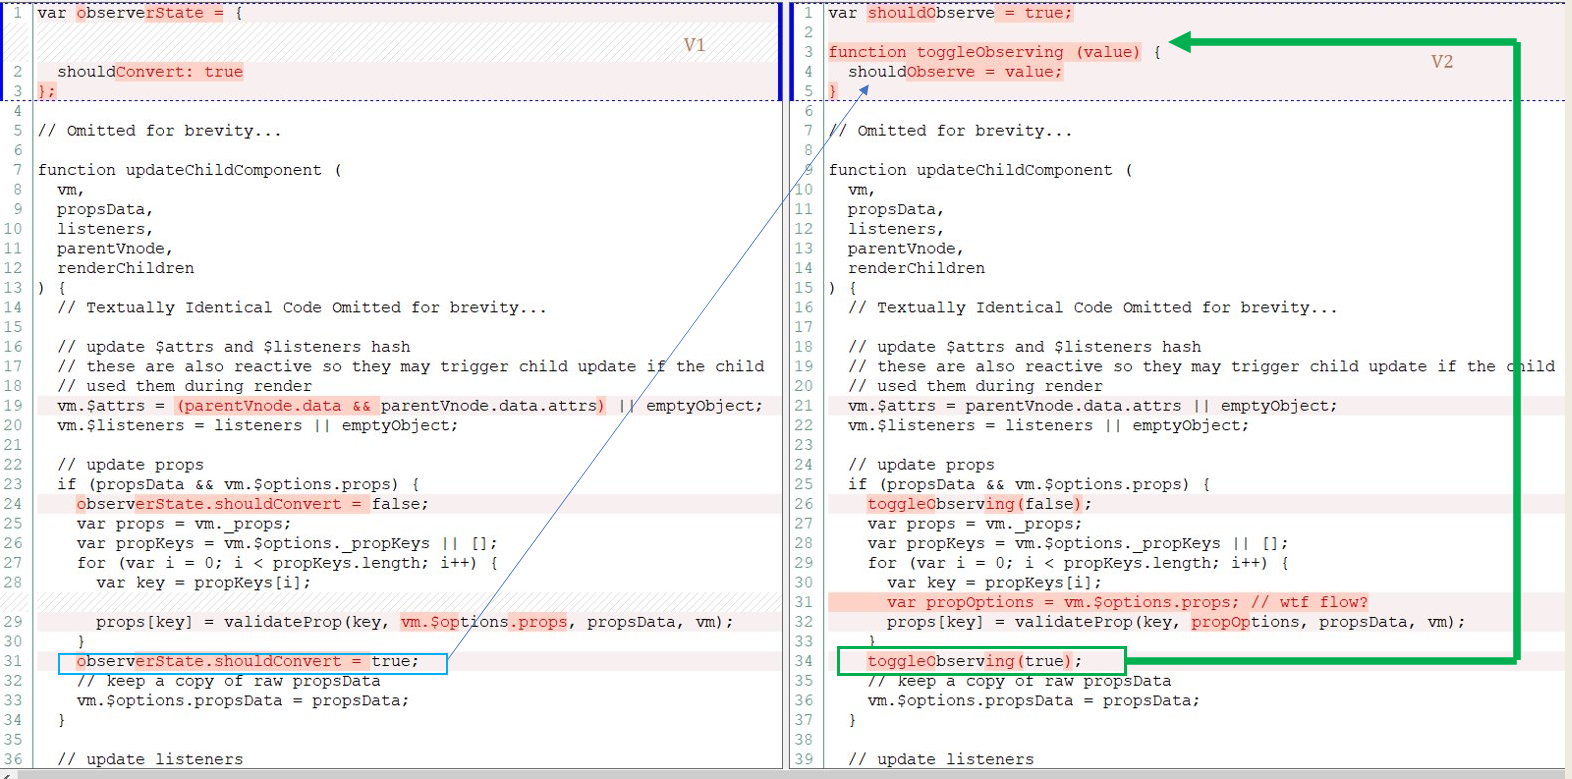
\includegraphics[width=\textwidth,height=\textheight,keepaspectratio]{extracttoggleObserving}
  \caption{Extract function toggleObserving from updateChildComponent}
   \label{fig:extractToggle}
\end{figure}



\subsection{RQ2: Accuracy on Detecting Variable Related Refactorings}

From \evTotalCommits{} commits, JsDiffer reported \renameVarTotalCount{} Rename Variable Refactorings. We validated \renameVarValidatedCount{} instances and calculated a precision of \renameVarPrecision{}\%.
We could not calculate recall as it is an extremely challenging and subjective task to find all the rename variable refactorings performed in a commit. However, our assumption is that most of the missed rename variable refactorings would be inside of a container expression which is currently poorly supported by JsDiffer.

In Addition to Rename Variable refactorings, we  also found Rename Parameter,  Add/Remove Parameter refactoring  instances. Only one Change Variable Kind refactoring was reported which turned out to be true positive.\nikos{I searched all your thesis and there is no definition or example about Change Variable Kind}

After taking a closer look at some of the false positives of Rename Variable refactorings, we have found that without static types, the syntax-aware replacement technique of RefactoringMiner does not perform very well in detecting variable level refactorings. This limitation was also mentioned in their paper. RefactoringMiner 2.0 relies heavily on types while detecting the signature of a method which helps find a pair of methods for comparison even after it has been renamed. This caused many false positives.


\subsection{RQ3: Performance Comparison}

RefDiff 2.0 outperforms JsDiffer in terms of execution time. Table \ref{table:performancecomparison} shows the execution time range for both tools. It took less than a second to detect refactorings in more than half of the commits for RefDiff 2.0. On the other hand, for the majority of the commits JsDiffer took 1 to 9 seconds to process them.

\begin{table}[!ht]
    \centering
    \caption{Execution Time Distribution over \evTotalCommits{} commits.}
    \begin{tabular}{|l|l|l|l|l|}
    \hline
        & \multicolumn{2}{|c|}{Commit Count} & \multicolumn{2}{|c|}{Percentage of Commits} \\ \hline
        Time Range (seconds) & JsDiffer & RefDiff 2.0 & JsDiffer & RefDiff 2.0 \\ \hline
        Less Than 1 & 202 & 340 & 33.22 & \bfseries 55.92 \\ \hline
        1 - 9 & 333 & 217 & \bfseries54.77 & 35.69 \\ \hline
        10 - 19 & 33 & 13 & 5.43 & 2.14 \\ \hline
        20 - 29 & 10 & 16 & 1.64 & 2.63 \\ \hline
        30 -59 & 23 & 17 & 3.78 & 2.80 \\ \hline
        Greater Than 60 & 7 & 5 & 1.15 & 0.82 \\ \hline
    \end{tabular}
    \label{table:performancecomparison}
\end{table}

We narrowed down the performance issue of JsDiffer into two phases: the parsing of source code and generation of source models, and the refactoring detection.

Both JsDIffer and RefDiff 2.0 are written in Java language. Both of them use Babel as the JavaScript source code parser in a virtual node.js environment. However, RefDiff 2.0 gets the source code back to the Java side in a tokenized format as a string where JsDiffer traverses the source code and passes back data from the JavaScript side to the Java Side for each node in the Abstract Syntax Tree. These multiple calls back and forth from Java to the JavaScript side turned out to be very costly and on average it took about 3 seconds to parse and create a model from a  commit.

On the other hand, the performance of detection of refactorings was degraded by Levensthein string distance calculation even though we have removed it for matching statements with container expressions. This occurs when having a large block of code inside an array access (e.g., arr[]) and the overall number of functions and statements is large.

\section{Limitations and Threats to Validity}
The reason behind such a low recall for JsDiffer is because RefactoringMiner employs a top-down approach when matching container elements where it checks the signature of two containers are similar, so that they are potential candidates for matching.

For example, if a class has more than half of its attributes matched with the same types, then our tool performs a diff between the classes similar to RefactoringMiner 2.0. However for JavaScript, since there are no types the only indicator is the name. So, if the name changes between two versions, the probability of finding a potential candidate to be matched with is reduced and since we do not employ a brute force approach JsDiffer missed many refactorings.


To remedy this problem, we currently check for child function names up to a nesting depth of 3. That means if two containers have similarly named functions inside their body or in their children/grandchildren's (up to depth 3) they are being considered for matching.

Unfortunately, this has proven to be highly inadequate for cases where the two containers do not contain any function declarations. In such a case, we cannot do the statement mapping because two differently named containers have no common function declarations and without static types, it's not possible to properly match the signature of the containers. This essentially became a Chicken and Egg problem where we want to do the statement mapping between two potential container elements but without the statement mappings sometimes it is not possible to find such candidate container pairs.

We do consider the name and number of the parameters during matching two function signatures. However,  due to the style of JavaScript code, we found that in many cases the whole program was written as a functional expression and assigned as a default value to the parameter. Therefore our approach can handle only simple cases and cannot generalize the structure yet.


As for the evaluation, even though we were careful when constructing our oracle, it is possible that we might have wrongly but unintentionally put the wrong validation. For example, whenever both tools reported the same refactoring, we considered it automatically as a True positive for both tools. However, we have found that in at least one case, both tools reported an Extract Function refactoring as Rename Function refactoring.

In addition,  JsDiffer by default processes files with .js extensions from a commit. It is very likely that a huge portion of the source code is left unprocessed which is typically found in .html, .jsx, or .ts file extensions. These files may contain vanilla  JavaScript,  TypeScript, JSX, or a mix of them. To reduce the scope we opted to not process other file extensions at this moment. 

Last but not the least, recall calculation for both tools suffer from the lack having all actually applied refactorings in the commit history.

%%%%%%%%%%%%%%%%%%%%%%%%
\chapter{Conclusion and future work}
\label{chap:conclusion}

In this thesis, we represent our tool JsDiffer which can detect Refactorings in JavaScript projects. We described our methodology and thoroughly discussed the difference between our tool and compared it with the current state-of-the-art RefDiff 2.0.

Our result showed that even though RefDiff 2.0 performed significantly better than JsDiffer, our approach was able to find some interesting refactorings that were missed by RefDiff 2.0. Especially our tool was able to find refactorings that were significantly structurally different. 

In summary, we learned the followings from this thesis:
\nikos{Add the general conclusion, as I discuss it in the email I sent to you on Sept 13th}
\begin{enumerate}
\item Though JsDiffer achieved a decent precision of \oraclePrecision{}\% in the oracle it has a low recall of \oracleRecall{}\%    for detecting JavaScript refactorings. 
\item JsDiffer achieved a precision of \renameVarPrecision{}\% on detecting Rename Variable refactorings.
\item RefDiff 2.0 also outperformed JsDiffer in execution as the majority of the commits were processed in under one second by RefDiff, while JsDiffer took 1-9 seconds to process the majority of the commits in the oracle.
\item JsDiffer was able to detect a single true positive instance of Change Variable Kind Refactoring.
\end{enumerate}
\nikos{You should discuss some potential improvements that can be made as future work}

%%%%%%%%%%%%%%%%%%%%%%%%%%%%%%%%%%%%%%%%%%%%%%%%
%% Bibliography
%%%%%%%%%%%%%%%%%%%%%%%%%%%%%%%%%%%%%%%%%%%%%%%%
\clearpage
\phantomsection
\addcontentsline{toc}{chapter}{Bibliography}  %  Add Bibliography to TOC
\singlespacing % save space in the bibliography
\bibliographystyle{unsrt}
\bibliography{references}



%%%%%%%%%% Appendices %%%%%%%%%%%%%%%%
% ---- Appendix settings. Please Do NOT change them. -----
\appendix
\setcounter{table}{0}		% reset the table counter
\setcounter{figure}{0}		% reset the figure counter
\renewcommand{\thefigure}{\Alph{chapter}.\arabic{figure}} 	% numbering the a figure in Appendix as Figure A.2, Figure B.1, etc.
\renewcommand{\thetable}{\Alph{chapter}.\arabic{table}}		% numbering the a table in Appendix as Table A.2, Table B.1, etc.

%%%%%%%%%% Body of Appendix %%%%%%%%%%%%%%%%
\begin{appendices}
\doublespacing

\chapter{Concordia Logos}
\label{chap:logos}
\begin{figure}[h!]
	\centering
	
\includegraphics{logos/Concordia_University_logo}
	\caption{Concordia University}
\end{figure}
\vspace{2em}
\begin{figure}[h!]
	\centering
	
\includegraphics{logos/Concordia_GinaCody_vertical}
	\caption{Gina Cody School of Engineering and Computer Science (vertical)}
\end{figure}
\vspace{2em}
\begin{figure}[h!]
	\centering
	
\includegraphics{logos/Concordia_GinaCody_horizontal}
	\caption{Gina Cody School of Engineering and Computer Science (horizontal)}
\end{figure}

\end{appendices}

\end{document}